\chapter{Herausforderungen im Frontend}
\label{cha:Herausforderungen im Frontend}

Im folgenden Abschnitt werden Herausforderungen im Frontend von My.PORTAL aufgezeigt. Diese Herausforderungen bilden wichtige Bewertungskriterien für die neue Komponentenbibliothek und die Einführung von Tailwind CSS.

\section{Redundante CSS Definitionen}
\label{sec:redundantCSS}
Das Frontendstyling wird seit Entwicklungsbeginn in SASS\footnote{ Syntactically Awesome Stylesheets (SASS) ist ein CSS Präprozessor } gestaltet. Jede Komponente wird als \textit{Single File Component}\footnote{ Vue Single File Components: \url{https://vuejs.org/v2/guide/single-file-components.html} } mit Component-Scoped CSS innerhalb der .vue Datei gestaltet. Es gibt keine globalen CSS-Klassen, die von mehreren Komponenten verwendete werden. Konstante Gestaltungswerte wie beispielsweise Abstände, Grids, Farben und komplexere Stylings werden per SASS-Mixins\footnote{ Mixins sind Styledefintionen die in ein Stylesheet eingefügt werden} oder SASS-Variablen eingefügt was zu redundanten Definitionen im transpilierten Code führt. 

\lstinputlisting[caption={UserList.vue (abstrakt)}, label={Redundante CSS Definitionen 1 - UserList.vue}]{code/003-000_herausforderungen/RedundanteCSSDefinitionen1.vue}

\lstinputlisting[caption={SiteNav.vue (abstrakt)}, label={Redundante CSS Definitionen 2 - SiteNav.vue}]{code/003-000_herausforderungen/RedundanteCSSDefinitionen2.vue}

\lstinputlisting[caption={Transpiliertes CSS Ergebnis}, label={Transpiliertes redundantes CSS}]{code/003-000_herausforderungen/transpiliertesErgebnis.css}

Die dargestellten Code Beispiele zeigen die Entstehung redundanter CSS-Definitionen. Zur weiteren Veranschaulichung des Problems wurden die gezeigten Mixins im Frontendcode gezählt und der daraus entstandenen Code kalkuliert. Neben den aufgelisteten Mixins gibt es noch 8 weitere Mixins, die mehr als drei mal verwendet werden.

\begin{itemize}
  \item \textbf{+make-container Mixin}: 37x verwendet [Desktop]\footnote{ Displaygrößen in welchen das Mixin verwendet wird }
  \item \textbf{+make-row}: 50x verwendet [Desktop]
  \item \textbf{+make-col-ready}: 69x verwendet [Desktop]
  \item \textbf{+make-col(*)}: 303x verwendet [Desktop, Tablet, Mobile]
\end{itemize}

Zu beachten ist, dass die Werte von \textit{+make-col(Parameter)} in verschiedenen Display-Kontexten greifen sollen und die Parameterwerte dabei von 1 - 12 (Integer) reichen können. Dies ist für die Berwertung in Abschnitt \ref{subsec:redundantCSS} relevant.
 
\section{Ungenutzte CSS Klassen}
\label{sec:unusedCSS}
Über die Entwicklungszeit hinweg hat sich gezeigt, dass es Komponenten gibt, die gegenüber ihrer ersten Ausführung geändert wurden. Dabei ist es passiert, dass ungenutzte CSS Klassen im Code verblieben sind und somit die Applikation unnötig vergrößern.

\section{Property Hell}
\label{sec:propertyHell}
Zu Beginn des Projektes wurden viele Komponenten spezifisch für den ersten Einsatzkontext entwickelt. Für ein konsistentes UI-Design war es immer wieder nötig bestehende Komponenten in einer abgewandelten Form im Portal wiederzuverwenden. Dazu wurden regelmäßig neue Properties zu Komponenten hinzugefügt, um sie an neue Kontexte anzupassen. Diese Properties steuern oft nur einen einzigen Usecase und erschweren es den Entwicklern die Dokumentation sowie den Code einer Komponente überblicken zu können. Besonders unübersichtlich ist es, wenn Komponenten das Verhalten von Kind-Komponenten per Properties verändern und ein Property durch verschiedenen Komponenten durchgereicht werden muss.

\begin{figure}[!ht]
	\centering
		%[natürliche Breite in Pixeln, natürliche Höhe in Pixeln, Abhängigkeit von der Textbreite]
		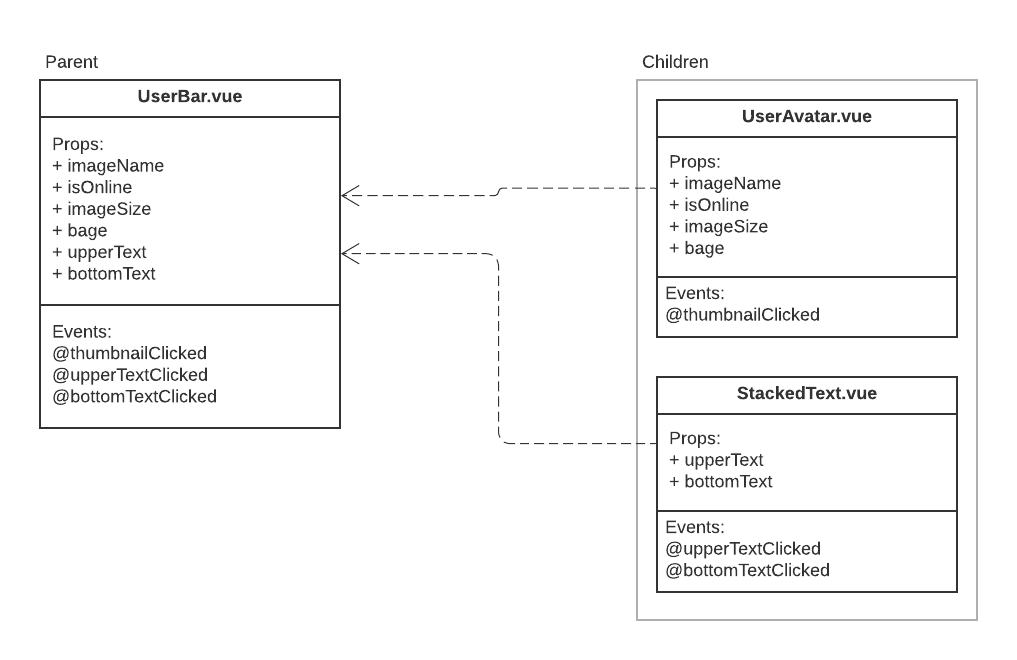
\includegraphics[width=0.75\textwidth]{images/003-000-001-property-hell.png}
	\caption{Abstraktes Beispiel der Property Hell}
	\label{fig:propertyHell}
\end{figure}

Abbildung \ref{fig:propertyHell} zeigt eine Eltern-Komponente die aus zwei weiteren Komponenten besteht. Property-Werte der Eltern-Komponente werden an Kinder-Komponenten weitergegeben. Je mehr Properties die Komponenten besitzen, desto unübersichtlicher wird der Code. Um das Beispiel nachvollziehbar darzustellen, wurden die Property-Namen und Events in allen Komponenten gleich genannt. In den orginallen Komponenten können Property-Namen voneinander abweichen und erschweren die Lesbarkeit und Nachvollziehbarkeit ein Komponente zusätzlich.
 
\section{Komponentenmanagement}
\label{sec:componentManagement}
Bisher wurden Komponenten gemäß dem Atomic Design Prinzip von \cite{AtomicDesign} entwickelt und geordnet. Dabei werden Komponenten in die Kategorien „Atom“, „Molekül“, „Organismus“, „Template“ und „Page“ kategorisiert. Hier haben sich für dieses Projekt zwei Schwächen herausgestellt:
\begin{enumerate}
 \item Der Unterschied zwischen Molekülen und Organismen ist oft für die Komponenten nicht strikt definierbar.
 \item Es kann passieren, dass größere Komponenten, wie beispielsweise Organismen Moleküle benötigen, die sonst keine andere Komponente benötigt. Diese Moleküle werden jedoch in dem Ordner Moleküle abgespeichert, was zu einer Unübersichtlichkeit der Repositories geführt hat. Der folgende Code soll dies veranschaulichen.
\end{enumerate}

\lstinputlisting[caption={components/organisms/Navigation/Navbar.vue}, label={Komponenten Management - Navbar.vue}]{code/003-000_herausforderungen/KomponentenMangement.vue}

\section{Post-Modularisierung von Komponenten}
\label{sec:postSplitting}
Es kommt immer wieder vor, dass Abschnitte einer Vue-Komponente zur Wiederverwendung eines Abschnitts in eine neue Komponente ausgelagert werden sollen. Neben der Herausforderung zugehörige Methoden und Variablen aus der Logik herauszufiltern müssen auch bereits spezifische Stylings in genisteten SASS-Abschnitten identifiziert und verschoben werden. Dies ist mühsam und fehleranfällig.

\section{Manuelle Dokumentation der Komponenten}
\label{sec:manualDocumentation}
Eine Dokumentation von Komponenten mit Code Beispielen und Property Auflistungen muss manuell vom Entwickler verantwortet werden. Dies führt dazu, dass Dokumentationen durch menschliche Fehler unvollständig, veraltet oder fehlerhaft sind. Zudem ist die manuelle Dokumentation aufwendig.
 
\section{Abhängigkeit der Portal-Konfiguration in portal-global-components}
\label{sec:portalConfigDep}
Jede Portal Instanz wird im portal-frontend-Repository konfiguriert und dort  gespeichert. Das Repository portal-global-components ist zur Verwendung auf eine gültige Portal-Konfiguration aus portal-frontend angewiesen. Dadurch sind die Komponenten in Zukunft nicht in anderen Projekten/Architekturen ohne eine solche Portal-Konfiguration nutzbar.
